% Chapter Template

\part {Search for heavy neutral leptons}


\chapter{Heavy Neutral Leptons} 
\label{Chapter3} 


In the Standard Model, all the fermions are known to have both, left and right handed chirality, the only exception comes from the neutrinos.

The recent neutrino oscillation experiments have clearly and definitely shown that neutrinos are massive; thus in this scenario, including the hypothesis of the existence of the right handed neutrinos, $\nu_{R}$ or \emph{Heavy Neutral Leptons} (HNLs), the light $\nu_{SM}$ flavor oscillations can be explained via the type I seesaw mechanism~\cite{MINKOWSKI1977421}~\cite{gellmann2013complex}~\cite{PhysRevLett.44.912}~\cite{PhysRevD.22.2227}.
Another strong possible endorsement comes from the possibility to consider the $\nu_{R}$ as part of the explanations for the baryon asymmetry of the universe; the mixing between $\nu_{R}$ violates \emph{CP} and the interaction of the $\nu_{R}$ may potentially generate a matter-antimatter asymmetry in the early stage of the formation of the universe~\cite{Canetti_2012}~\cite{KUZMIN198536}.

These few examples, which are going to be explored later on, show already the relevance and the interest of the HNL program and the strong motivations behind the existence of the $\nu_{R}$. This huge enthusiasm has lead in the past $\sim10$ years to the creation of a very active community with strong synergy between the theory people and the experimental collaborations which has brought to the publication of an impressive numbers of papers and the proposal of a consistent number of experiments focused manly on heavy neutral leptons. 

\section{Neutrino Portal} \label{sec:neutrinoPortal}
The \emph{neutrino portal} is determined as coupling of one or more dark fermions $N$ ($N_{I} = 1,2,...$ $\mathcal{N}$), which are sterile with respect to the SM gauge interactions, to the gauge-invariant operator ($\bar{L}_{\alpha}  \cdot \widetilde \Phi$); the general form of the neutrino portal could be displayed as: 
\begin{equation}
\label{eq:neutrinoportal}
\mathcal{L}_{vector} = \mathcal{L}_{SM} + \mathcal{L}_{DS} + \sum F_{\alpha I} (\bar{L}_{\alpha}  \cdot \widetilde \Phi)N_{I} + h.c.
\end{equation}

where the summation loops over the flavor of lepton doublets ${L}_{\alpha}$ ( $\alpha = e,\; \mu, \: \tau$) and the number of available HNLs $N_{I}$; $F_{\alpha I} $ are the Yukawa couplings and $\Phi$ is the Higgs doublet. The term $\mathcal{L}_{DS}$ should contain the mass term of HNL which can be both Majorana or Dirac~\cite{Alekhin_2016}.
Fixing the $\Phi$ to its vacuum expectation value, $\widetilde \Phi = \frac{1}{\sqrt{2}} \binom{v}{0}$, and diagonalize the mass term of the dark fermions, the last term in Eq.~\ref{eq:neutrinoportal} brings to the quadratic mixing of the neutrinos $\nu_{\alpha}$ with the $N_{I}$; this mixing is parametrized by a matrix $V.$ In the minimal HNL models, the elements of the matrix $V$ control both the production and the decay of the HNLs (see fig.~\ref{fig:c3diagram_decay}). 
If $\mathcal{N} = 3$, there is a right-chiral counterpart for each $\nu_{SM}$, see fig.~\ref{fig:c3sm_extension}. The fermion $N_I$ can have mass $M_I$ which is independent  of the value of $F_{\alpha I}$.
\begin{figure}[t!]
  \centering
  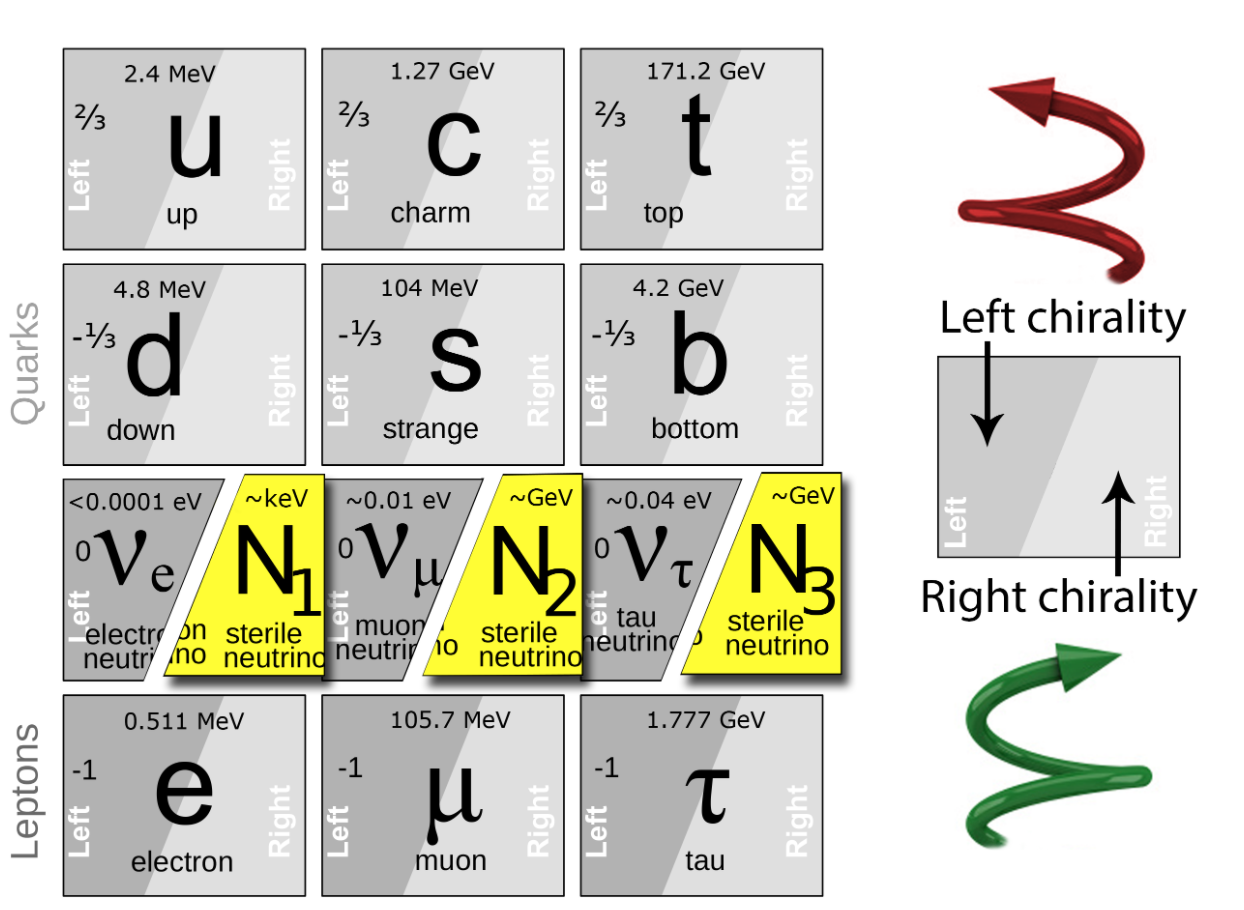
\includegraphics[width=.60\textwidth]{Figures/c3/SM_extension}
    \caption{There are 3 SM neutrinos $\nu_{e}, \; \nu_{\mu}, \;\nu_{\tau}$ which are massless and always left-chiral; 3 right-chiral counterparts are added $N_{1}, \; N_{2}, \;N_{3}$. They are sterile so they do not feel the electric, weak and strong forces}
  \label{fig:c3sm_extension}
\end{figure}

Considering the existing searches and considering a model-indipendent phenomenological approach, we could assume the existence of only a \emph{single} light HNL which is light enough to be kinematically accessible at the accelerator experiments; see full overview in~\cite{Atre_2009}. 

There are then only two free parameters to be constrained: the mass $M_I$ of the HNL and its coupling with the SM neutrino of flavor $\alpha$ controlled by the Yukawa coupling $F_{\alpha I}$. Without any signal excess, upper limits are settled on the mixing parameter $|V^2_{\alpha I}|$ ($= |F^2_{\alpha I}|$) as function of the $M_I$ for a given flavor $\alpha$. It is frequently assumed that in the matrix $V$ the other mixing elements for the residual flavors are zero; this latter consideration, in spite of the fact that does not translate into a valid concrete model, it is very useful to extract generic limits on the single $|V^2_{\alpha I}|$ without involving any model dependent hierarchy between the different flavor mixings. 
\begin{figure}[h]
  \centering
  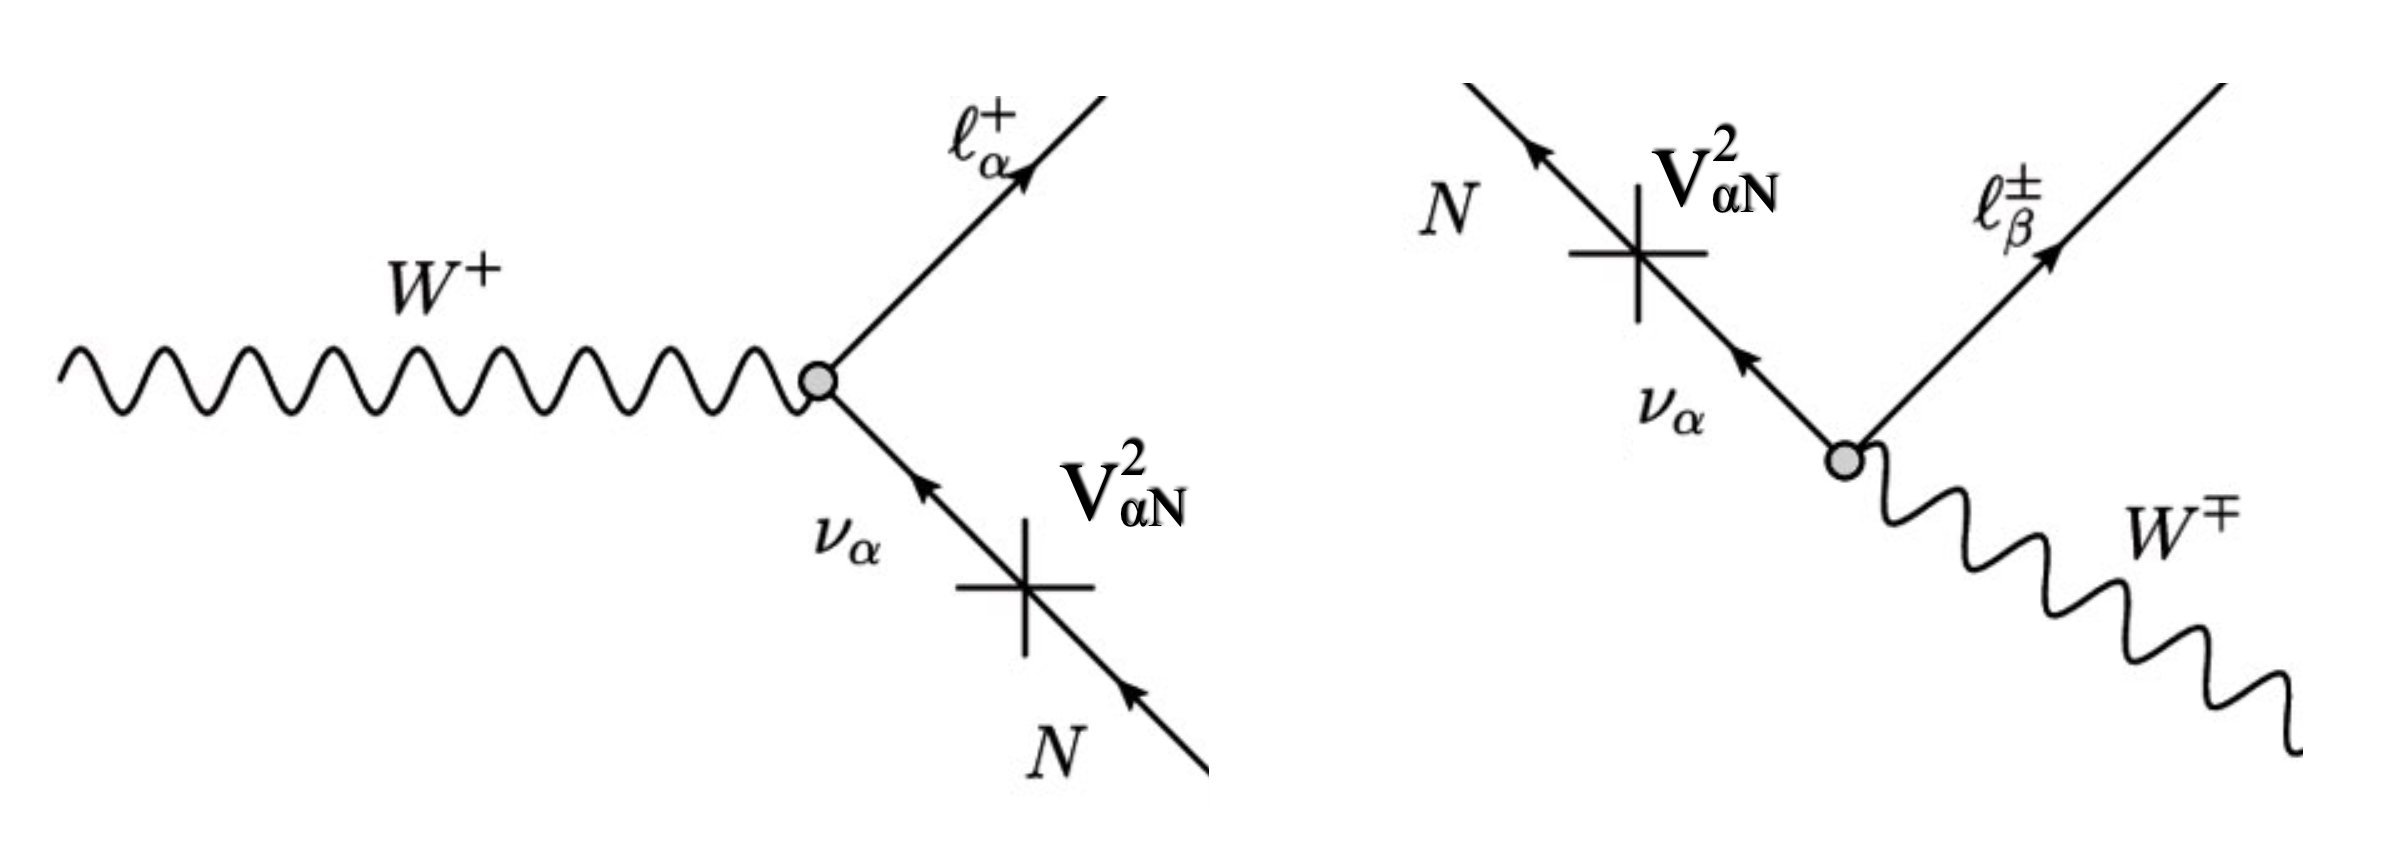
\includegraphics[width=.80\textwidth]{Figures/c3/diagram_decay}
    \caption{Production (left) and decay (right) of the particle $N_{I}$.}
  \label{fig:c3diagram_decay}
\end{figure}

\section{Heavy neutral lepton formalism and extension of the standard model}
To set up our notation and convention, we first discuss the formalism for the simplest
extension of the SM which includes right handed singlets. In the next section (~\ref{sec:currentlimits}), we will try to contextualize the theory, here explained, summarizing the current constraints on the mass and mixing of a heavy neutrino from various direct
detection experiments, accelerator searches and electroweak precision constraints.
\subsection{Seesaw mechanism}\label{sec:seesaw}
The most general renormalisable Lagrangian for the neutrino masses includes both the Dirac and Majorana mass terms. The SM Lagrangian $\mathcal{L}_{SM}$ is extended adding $\mathcal{N}$ right-handed neutrinos $N_I$: (for notations see Eq.~\ref{eq:neutrinoportal}).
\begin{equation}
\label{eq:fullSMLag}
 \mathcal{L} = \mathcal{L}_{SM}+ i \bar N_I \partial_\mu \gamma^\mu N_I -
  \left(F_{\alpha I} \,\bar L_\alpha N_I \tilde \phi 
    - \frac{M_I}{2} \; \bar {N_I^c} N_I + h.c.\right)
\end{equation}
As already explained in the previous section (~\ref{sec:neutrinoPortal}), these $N_I$ are neutral with respect to all the gauge interactions of the SM, thus are called \emph{sterile neutrinos} or \emph{gauge-singlet fermions}.
In the Higgs phase, the term~\ref{eq:neutrinoportal} brings to the $\nu_{\alpha} - N_I$ mixing. As result the \emph{charge eigenstates} of the $\mathcal{L}_{SM}$ (~\ref{eq:fullSMLag}) do not coincide with the \emph{mass eigenstates}, which can be extracted diagonalizing the following matrix:
\begin{equation}
\label{eq:matrixmass}
 \mathcal{M}_{\nu,N} = 
\begin{pmatrix}
0 & m_D\\
m^{T}_{D} & M_I
\end{pmatrix}
\end{equation}
with $m_D = 3 \times  \mathcal{N}$ Dirac mass matrix, $(m_D)_{\alpha I} = F_{\alpha I}v, \; v = \sqrt{2}\langle \Phi \rangle$ and $M_I$ is $\mathcal{N} \times \mathcal{N}$ matrix of Majorana masses.

Considering the relation between $M_I$ and $m_D$, we could explore two interesting extreme limits:
\paragraph {Pure Majorana neutrino, $m_D \ll M_I$.}
In this limit, the mass matrix give rise to 3 almost pure right-handed neutrinos with heavy Majorana mass $M_I$ and 3 almost pure left-handed neutrinos with light Majorna mass $m_\nu = - (vm_D)^{T}M^{-1}_{I}(vm_D)$ which are the 3 eigenvalues of the matrix $(\mathcal{M}_{\nu})_{\alpha \beta}$. This mechanism is then referred to as the \emph{seesaw mechanism}\footnote{This mechanism is usually called \emph{Type-I seesaw}. \emph{Type-II seesaw} has an extra SU(2) triplet scalar~\cite{Deppisch_2015}; in \emph{Type-III seesaw} an extra fermion in the adjoint of SU(2) is added to the model~\cite{Foot:1988aq}}~\cite{MINKOWSKI1977421}~\cite{Mohapatra:1979ia}~\cite{Yanagida:1979as}.
\begin{figure}[h]
  \centering
  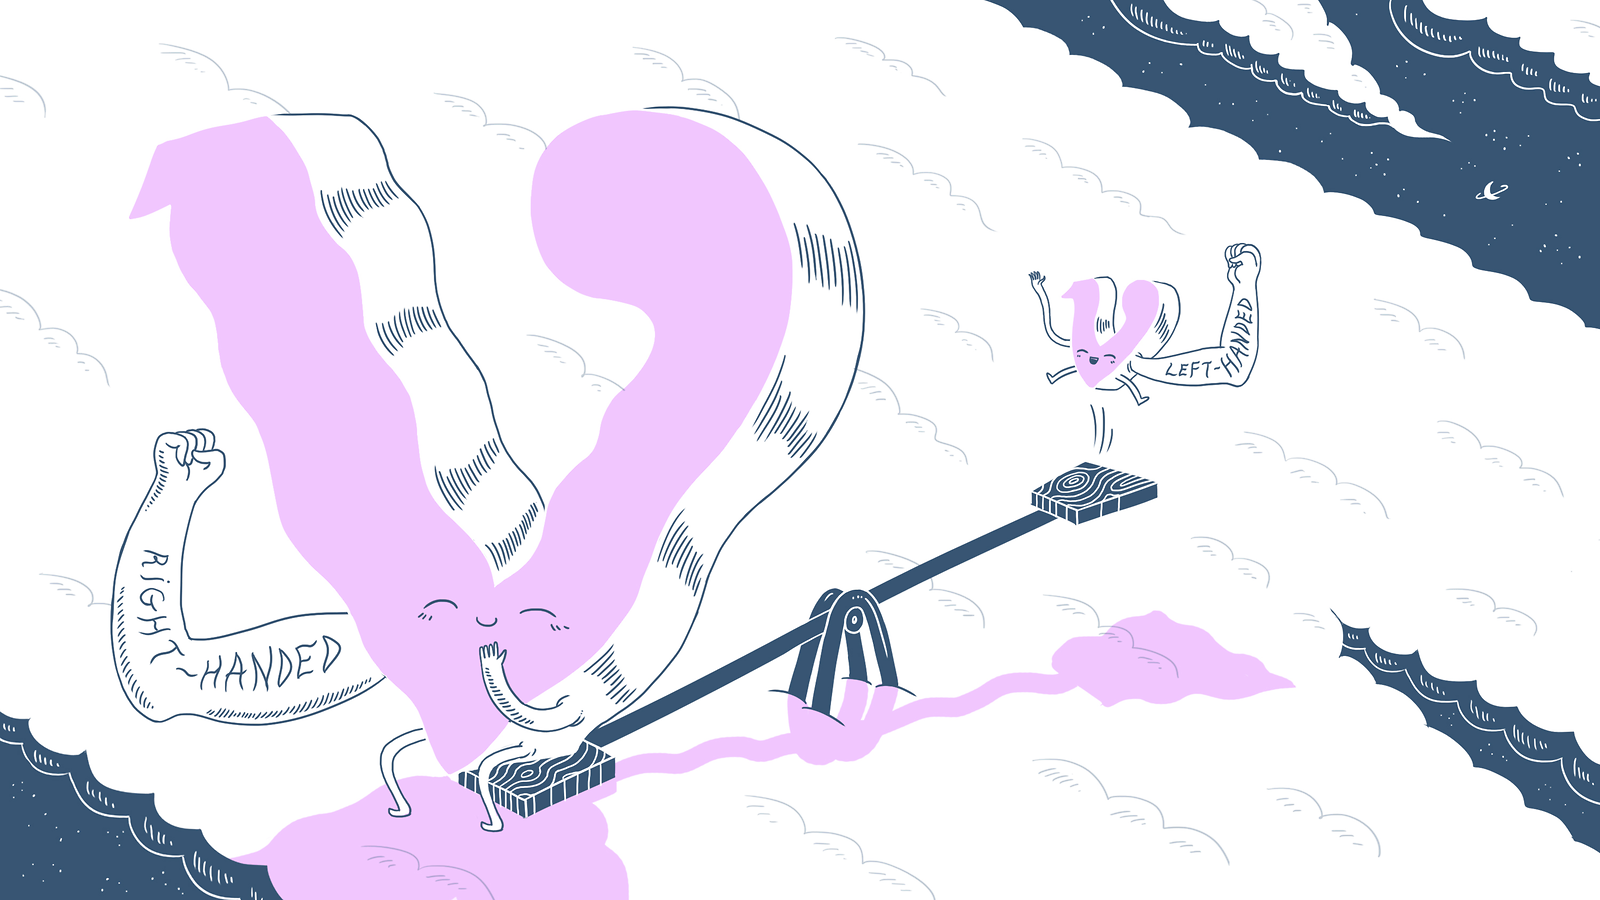
\includegraphics[width=.60\textwidth]{Figures/c3/funny.png}
    \caption{Silly representation of the \emph{seesaw mechanism}~\cite{funny}. Note that for a fix value of $m_D$, higher is value of the $m^{R}_I$ lower is the one of the $m^{L}_I$ and vice-versa, from this the \emph{seesaw} name.}
  \label{fig:c3funny}
\end{figure}
There are then the other $\mathcal{N}$ eigenstates of the $\mathcal{M}_{\nu,N}$ which almost coincide with the $N_I$ up to a small admixture of $\nu_\alpha$.
The magnitude of this mixing is given by the ratio of the Dirac and Majorana masses $\rightarrow$ \emph{mixing angle} or \emph{active-sterile mixing}:

\begin{equation}
\label{eq:v2}
 V^2_{\alpha I} \equiv \frac{v^{2}|F_{\alpha I}|^2}{M^{2}_{I}} \ll 1
\end{equation}
It generates the 9 measurable neutrino mass parameters from $m_D$ and $M_I$, that contain 18 unknown parameters to the Lagrangian: $number\; of \; HNL \; parameters = 7 \times \mathcal{N} - 3$. $\mathcal{N}$ are the real Majorana masses $M_I$ plus $3\times \mathcal{N}$ complex Yukawa coupling $F_{\alpha I}$ minus 3 phases which go to the redefinitions of $\nu_e, \; \nu_\mu,\; \nu_\tau$.

\paragraph {Pure Dirac neutrino, $M_I \ll m_D$.}
In this limit, the mass matrix give rise to 3 Dirac neutrinos $\Psi = (\nu_L,\:\bar{\nu_R})$ with masses $m_\nu = m_D$. To obtain the observed neutrino masses the coupling is needed to be $F_{\alpha I} \sim 10^{-12}$ which is much smaller than the SM Yukawa couplings.

\vspace{5mm} 
\subsection{Considerations on Majorana and Dirac neutrinos}
These paragraphs below are freely inspired by the overview given by R.D. Kauber here~\cite{webpage_seesaw}.
\subsubsection {Distinction between Majorana and Dirac terms.}
The nomenclature "Majorana" is used to define different things and it is important for the following chapters to clarify the meaning.

In the Sec.~\ref{sec:seesaw} \emph{Majorana} and \emph{Dirac} are used to refer to the mass terms in the Lagrangian~\ref{eq:fullSMLag}. The additional meaning is related to the type of neutrino. A \emph{Majorana} particle is defined as a particle that is its own antiparticle.  A Dirac particle has an antiparticle that is distinctly different from it. Neutrino are the only particle which can be both \emph{Majorana-Dirac} while all the other fermions are strictly Dirac-type. 

\subsubsection{Lepton Number conservation.}
To be more clear and explicit, we write the Dirac mass term as:
\begin{equation}
\label{eq:dirac}
-m_D (\bar{\nu_L}\nu_R + \bar{\nu_R}\nu_L)
\end{equation}
and the Majorana one:
\begin{equation}
\label{eq:majorana}
-\frac{1}{2}m^{L}_{I}(\bar{\nu_L}\nu^{c}_L + \bar{\nu_L}^{c}\nu_L) -\frac{1}{2}m^{R}_{I} (\bar{\nu_R}\nu^{c}_R + \bar{\nu_R}^{c}\nu_R)
\end{equation}
In this way is it easier to see the interactions: $\nu_L$ destroys a left-handed (LH) neutrino and creates a right-handed (RH) $\bar{\nu_R}$, $\bar{\nu_L}$
 creates a LH neutrino and destroys a RH $\bar{\nu_R}$, $\nu^{c}_L$ creates a LH neutrino and destroys a RH antineutrino, $\bar{\nu}^{c}_L$ destroys a LH
 neutrino and creates a right-handed antineutrino.

Looking now at the Feynman diagram of the first term of
Eq.~\ref{eq:dirac} a RH particle disappears at a point and a LH
particle appears. Therefore weak (chiral) charge is not conserved, but
the lepton number, however, is conserved, as we started with a
neutrino (not an anti-neutrino) and ended up with a neutrino
$\rightarrow$ \textbf{Dirac neutrinos conserve the lepton number}.

Same considerations can be made for the Eq.~\ref{eq:majorana}, the
weak charge is not conserved and neither the lepton number. We started
with zero neutrinos and ended up with two neutrinos. $\rightarrow$
\textbf{Majorana neutrinos violate the lepton number}.

Considering here (Fig.~\ref{fig:c3hnldiagram}) as example the leptonic decay of the \PW boson from the HNL decays, if the HNL is of Majorana nature, $\ell$ and $\ell^\prime$ (or $\ell$
and $\nu_{\ell^\prime}$) can either have the same chirality
(Fig.~\ref{fig:c3hnldiagram} left) or opposite chirality
(Fig.~\ref{fig:c3hnldiagram} right). The former decay represents a case
of lepton-number violation (LNV), while the latter decay conserves the
lepton number (LNC).
In the case of a HNL decay mediated by a $\PW^\ast$ boson, a LNV decay
(Fig.~\ref{fig:c3hnldiagram} top left)
can lead to final states with no opposite-sign, same-flavor lepton
pairs (no-OSSF), such as $\Pe^\pm\Pe^\pm\PGm^\mp$ or
$\PGm^\pm\PGm^\pm\Pe^\mp$.
Decays mediated by a $\PZ^\ast$ boson (Fig.~\ref{fig:c3hnldiagram}
bottom) and LNC decays (Fig.~\ref{fig:c3hnldiagram} right), instead, are
always accompanied by an opposite-sign, same-flavor lepton pair
(OSSF).

The HNL can couple exclusively to a single lepton-neutrino family
(\ie only one of \mixpare, \mixparm, or \mixpart is nonzero)
or to multiple families (\ie at least two of \mixpare, \mixparm,
and \mixpart are nonzero at the same time).
In the former case, $\ell$ and $\ell^\prime$ (or
$\nu_{\ell^{\prime}}$) always belong to the same lepton generation,
and the lepton flavor is conserved (LFC).
If \hnl couples to multiple lepton families instead, then the
lepton flavor can be violated, $\ell\neq\ell^\prime$ (LFV).
In the LFV case, decay rates to different flavors might not be the
same ($\mixpare,\mixparm,\mixpart>0$, but
$\mixpare\neq\mixparm\neq\mixpart$).

\begin{figure}
\centering
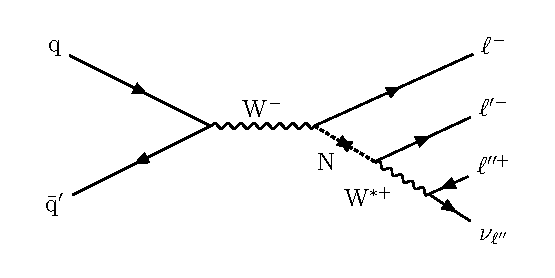
\includegraphics[width=0.48\textwidth]{Figures/c3/hnl_feyn.pdf}
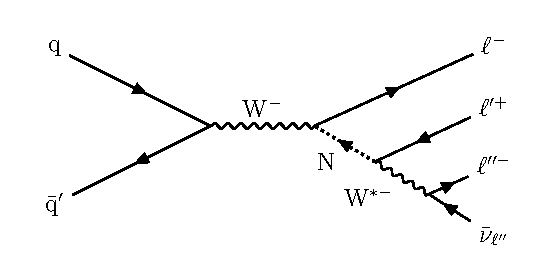
\includegraphics[width=0.48\textwidth]{Figures/c3/hnl_feyn_2.pdf}\\
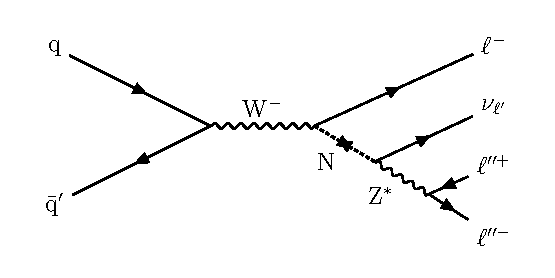
\includegraphics[width=0.48\textwidth]{Figures/c3/hnl_z_feyn.pdf}
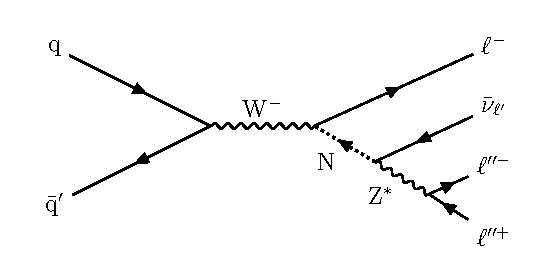
\includegraphics[width=0.48\textwidth]{Figures/c3/hnl_z_feyn_2.pdf}
\caption{Typical diagrams for the production of a HNL at the LHC 
($\hnl$) through its mixing with a SM neutrino, leading to a
final state with three charged leptons and a neutrino.
The HNL decay is mediated by either a $W$ (top row) or a $Z$ (bottom
row) boson.
In the diagrams on the left, $\hnl$ is assumed to be a Majorana
neutrino, thus $\ell$ and $\ell^\prime$ in the $W^\ast$-mediated
diagram (top) can have the same electric charge, with lepton-number
violation (LNV).
In the diagrams on the right instead, the $\hnl$ decay conserves the
lepton number (LNC) and can be either a Majorana or a Dirac
particle. Therefore $\ell$ and $\ell^\prime$ in the
$W^\ast$-mediated diagram (top right) have always opposite charge.
If \hnl couples exclusively to a single lepton-neutrino generation,
then $\ell$ and $\ell^\prime$ (or $\nu_{\ell^{\prime}}$) always belong
to the same lepton generation, and the lepton flavor is conserved
(LFC). If \hnl couples to multiple lepton families instead, then the
lepton flavor can be violated, $\ell\neq\ell^\prime$ (LFV).}
\label{fig:c3hnldiagram}
\end{figure}


\subsubsection{Decay width and branching ratio}
The main consideration and difference between Majorana and Dirac is that in the first case \hnl particle is defined as a particle that is its own antiparticle. This implies that both $N_I\rightarrow \PW^{+}\ell^-$, $\PZ\nu_{\ell}$, $H\nu_{\ell}$ and $N_I\rightarrow \PW^{-}\ell^+$, $\PZ\bar{\nu}_{\ell}$, $H\bar{\nu}_{\ell}$ decay modes are open. This means that the partial width of $N_I\rightarrow \PW^{+}\ell^-$ and $N_I\rightarrow \PW^{-}\ell^+$ have the same value. Thus the total width for a Majorana neutrino and a Dirac neutrino fixing the mass are related by:
\begin{equation}
\label{eq:width}
\Gamma^{Tot, \: Majorana}_{N_{I}} = 2 \times \Gamma^{Tot, \: Dirac}_{N_{I}}
\end{equation}
This brings to the relationship between the life time:
\begin{equation}
\label{eq:lifetime}
c\:\tau^{Tot, \: Majorana}_{N_{I}} = \frac{1}{2} \times c\:\tau^{Tot, \: Dirac}_{N_{I}}
\end{equation}

\subsection{Prompt and long-lived HNL}\label{sec:promptll}

The lifetime of a HNL is strongly dependent on $M_{N_I}$ and $|V_{\alpha I}|^2$,
and increases rapidly at small masses and low values of the mixing
parameter (see Fig.~\ref{fig:hnlLifetime}):
\begin{equation}
\label{eq:lifetimedependences}
c\:\tau_{N_{I}} \propto\mathrm{M_{N_I}^{-5}|V_{\alpha I}|^{-2}}
\end{equation}
As a consequence, the kinematics and acceptance of HNLs with masses
below about 20 GeV are significantly affected by their long lifetimes,
and must be accounted for in the signal simulation and in the result
interpretation.
If $\hnl$ has a long lifetime, in particular, its decay products
($\ell^{\pm\prime}$, $\ell^{\mp\prime\prime}$, $\nu_{\ell^{\prime\prime}}$ or
$\nu_{\ell^{\prime}}$, $\ell^{\pm\prime\prime}$, $\ell^{\mp\prime\prime}$, see Fig.~\ref{fig:c3hnldiagram})
emerge from a secondary vertex, spatially displaced with respect to
the primary vertex of the process, and distinguishable from it.
\begin{figure}
\centering
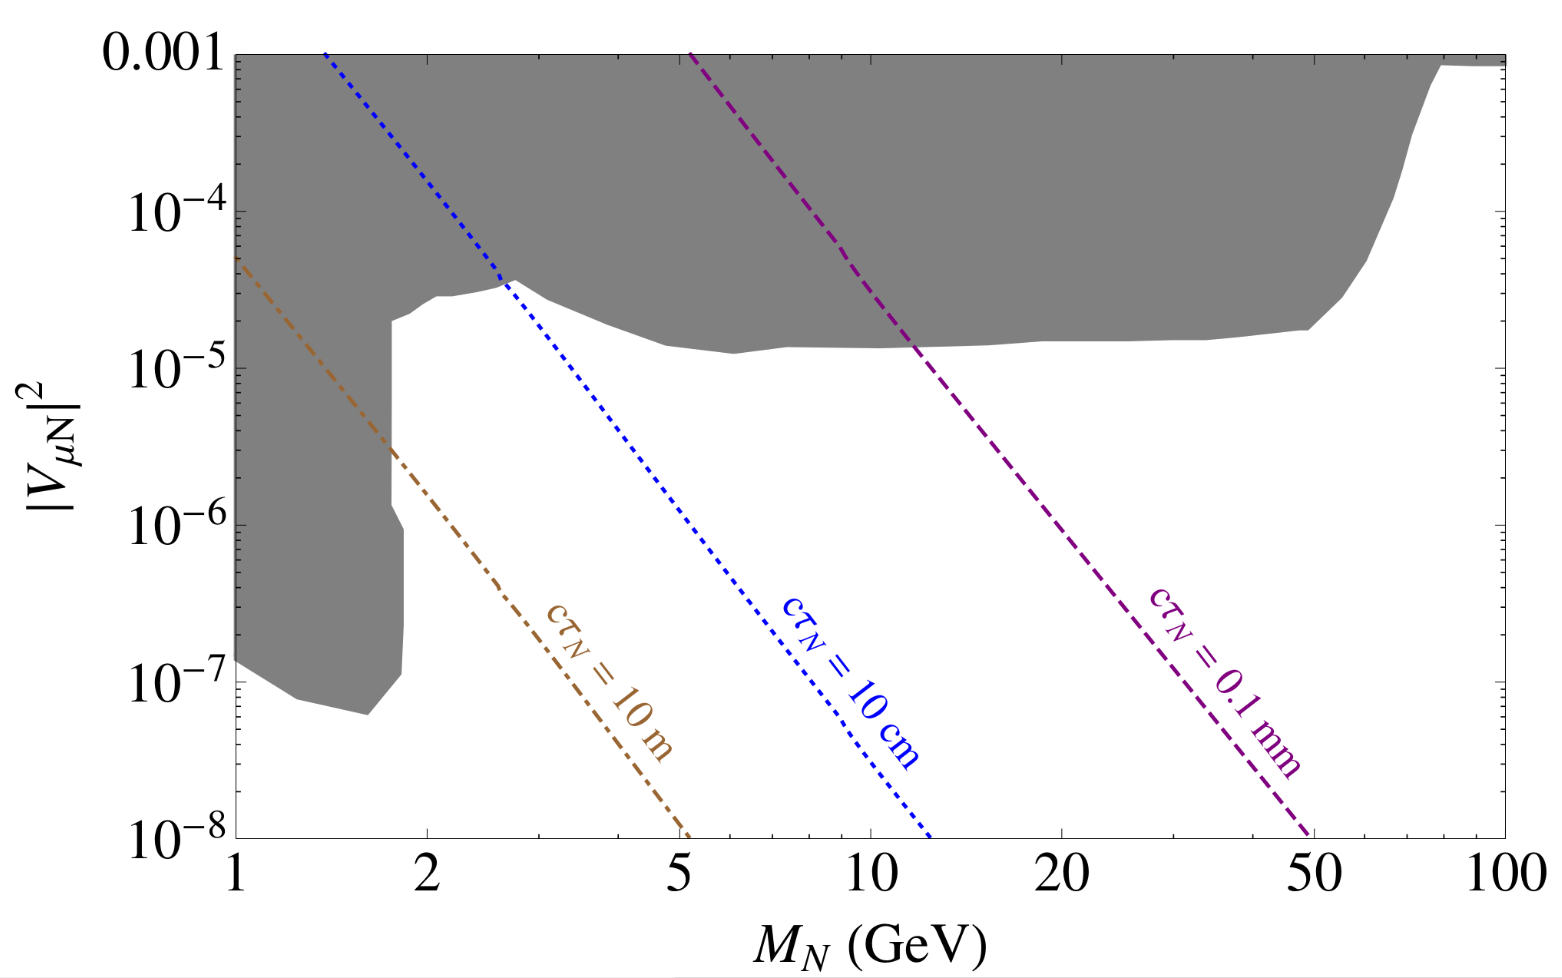
\includegraphics[width=0.78\textwidth]{Figures/c3/graph_displ.png}
\caption{Lifetime $c\tau$ of a HNL as a function of its mass \mhnl
and its mixing parameter \mixpar to a single lepton family:
the three oblique lines correspond to $c\tau$ values of (from left to
right) 10~m,  10~cm, and 0.1~mm.
The shaded grey area represents---approximately---the region of the
parameter space excluded by previous searches.}
%% If $\hnl$ has a long lifetime, its decay products emerge from a
%% secondary vertex, distinguishable from the primary vertex of the
%% process.}
\label{fig:hnlLifetime}
\end{figure}


%%%%%%%%%%%%%%%%%%%%%%%%%%%%%%%%%%%%%%%%%%%%%%%%%%%%
%%%%%%%%%%%%%%%%%%%%%%%%%%%%%%%%%%%%%%%%%%%%%%%%%%%%
%%%%%%%%%%%%%%%%%%%%%%%%%%%%%%%%%%%%%%%%%%%%%%%%%%%%
\vspace{5mm} 
\section{Theoretical and experimental constraints} \label{sec:currentlimits}
For a complete overview of the theoretical and experimental constraints of sterile neutrinos searches see Ref~\cite{Deppisch_2015},~\cite{10.3389/fphy.2018.00040},~\cite{PhysRevD.78.013010},~\cite{Drewes_2017},~\cite{DREWES2017250} and~\cite{Antusch_2014}.


Sterile neutrinos mix with the $\nu_{SM}$, thus at small mixing the
active-neutrino mass states contain a small part of sterile neutrinos. Consequently, the mass eigenstates in the HNL couple to SM particles thanks to the tiny but nonzero mixing $V_{\alpha I}$, Eq.~\ref{eq:v2}.

In principle, in any weak processes where the $\nu_{SM}$ participates, also the HNLs do. The strength is suppressed due to the smallness of the $\nu_\alpha - N_I$ mixing angle but the kinematics properties could show the interaction due to the fact that the HNL is much more massive than the active-neutrino.
Therefore, it is possible to select a particular channel and phase space which enhances some kinematics features associated to the presence of the sterile neutrino.

These properties are explored and exploited in the direct searches for HNLs.



\subsection{Direct HNL searches}
Considering the wide theoretical accessible mass ranges (MeV-TeV ) and taking into account
the several production and decay modes, we have a quite rich
experimental landscape. 
\begin{itemize}
\item For $M_N$ values below 1 MeV, HNL can be probed by
  neutrino-oscillation experiments~\cite{de_Gouv_a_2005};
\item for 10 eV $< M_N <$ 1 MeV, searches for
  $0\nu\beta\beta$ and precision measurement of $\beta-$decay energy
  spectra have constrained the mixing \mixpare~\cite{PhysRevLett.111.122503};
\item for 1 MeV $< M_N <$ 1 GeV, both \mixpare and \mixparm have been
  constrained by \emph{peak searches} using leptonic decay of pions
  and kaons like $K \rightarrow \mu(e) N$, $\pi \rightarrow \mu(e)
  N$~\cite{Liventsev_2013};
\item for HNL in the MeV-GeV mass ranges, many searches through
  sterile neutrino decay products have been performed at beam dump experiments~\cite{DORENBOSCH1986473};
\item for HNL in the GeV-TeV mass ranges, we enter in the domain of
  the leptonic and hadron colliders.
\end{itemize}

Quite often the HNL bounds are shown in the 2D plane $V_{\alpha N} \longleftrightarrow
M_N$ with the assumption to fix at zero the other mixing angles which are not
represented in the plot. 

To have a clear overview of the current experimental (and theoretical)
limits we can refer to
Figs.~\ref{fig:HNL_bc6_pbc_2},~\ref{fig:HNL_bc7_pbc_2}
and~\ref{fig:HNL_bc8_pbc_2}. Filled colored areas show the existing
limits which, for low masses (below the charm mass), are driven by the
results from beam dump experiments (PS191 and CHARM); for masses above
the charm mass, the most stringent limits are the ones coming from LEP
(DELPHI) and from Belle and most recently from CMS and ATLAS.



\begin{figure}[h]
  \centering
  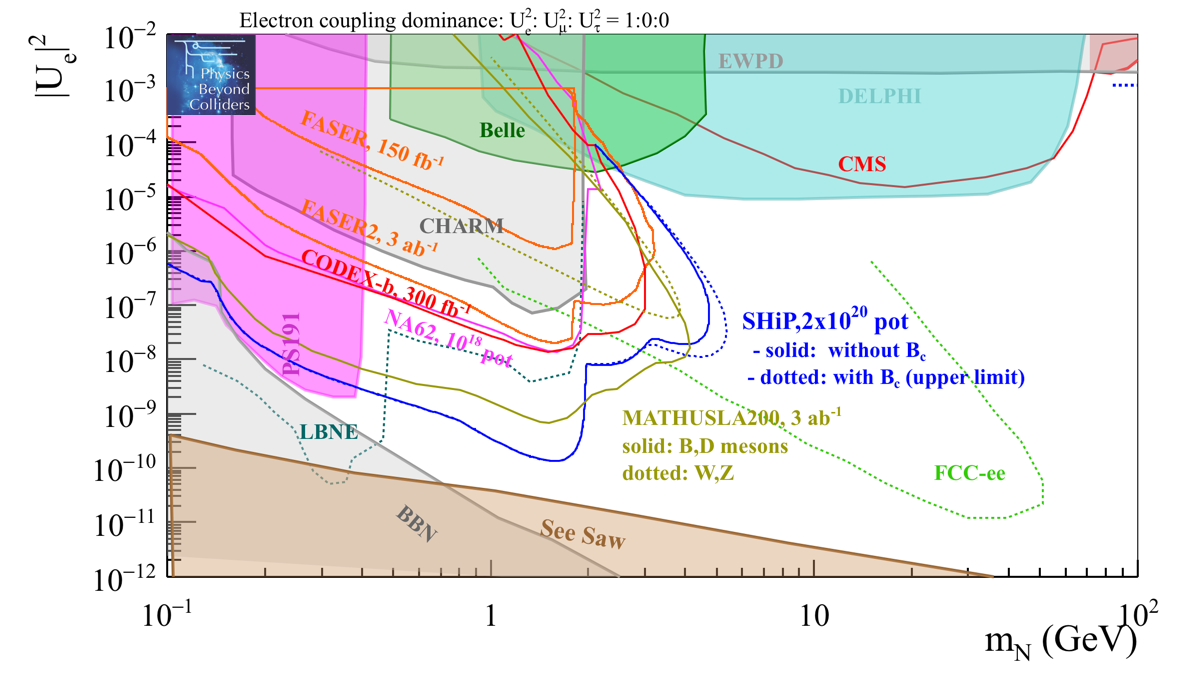
\includegraphics[width=.90\textwidth]{Figures/c3/HNL_bc6_pbc_2.png}
    \caption{Sensitivity to HNL with coupling to $\nu_e$ only. Current bounds (filled areas) and 10-15 years prospects for projects
(SHiP, MATHUSLA200, CODEX-b and FASER2) (solid lines). Projections for a LBNE
near detector with $5\times 10^{21}$ pot and from FCC-ee with
$10^{12}$ $\PZ_0$ decays are also shown.
The gray contour named "BBN'' corresponds to and HNL lifetime $>1$sec,
which is disfavored by BBN~\cite{Ruchayskiy_2012}. The brown line
labeled "seesaw'' represents the scale of mixing in general expected
in the canonical \emph{seesaw }. The very light gray at the top
labeled as "EWPD'' is the 90\% C.L. exclusion limit from the
electroweak precision data~\cite{Antusch_2015}. The other solid
contours are explained in the paragraph. 
% The green contour labeled "Belle'' is the exclusion
%region at 90\% C.L from HNL searches in B-meson decays at
%Belle~\cite{Liventsev_2013}. Those labeled "PS191'' (magenta) and
%"CHARM' (gray) are excluded at 90\% C.L. from beam-dump experiments.
}
  \label{fig:HNL_bc6_pbc_2}
\end{figure}

\begin{figure}[h]
  \centering
  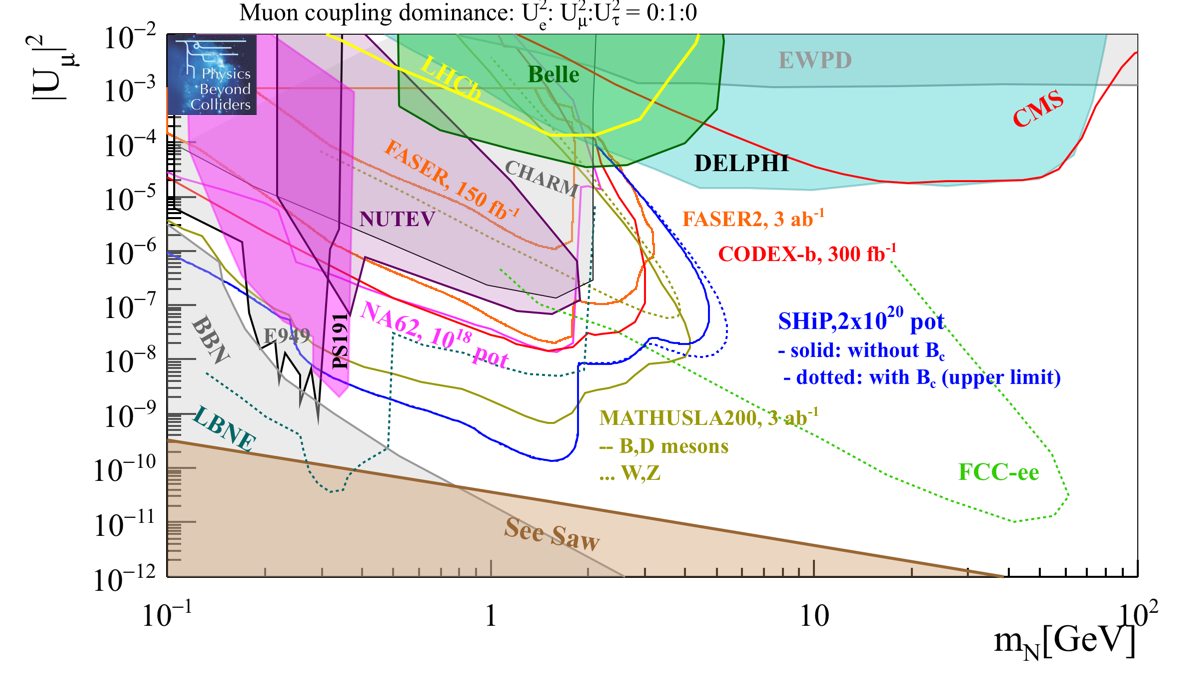
\includegraphics[width=.90\textwidth]{Figures/c3/HNL_bc7_pbc_2.png}
    \caption{Sensitivity to HNL with coupling to $\nu_\mu$ only. Current bounds (filled areas) and 10-15 years prospects for projects
(SHiP, MATHUSLA200, CODEX-b and FASER2) (solid lines). Projections for a LBNE
near detector with $5\times 10^{21}$ pot and from FCC-ee with $10^{12}$ $\PZ_0$ decays are also shown. The gray contour named "BBN'' corresponds to and HNL lifetime $>1$sec,
which is disfavored by BBN~\cite{Ruchayskiy_2012}. The brown line
labeled "seesaw'' represents the scale of mixing in general expected
in the canonical \emph{seesaw }. The very light gray at the top
labeled as "EWPD'' is the 90\% C.L. exclusion limit from the
electroweak precision data~\cite{Antusch_2015}. The other solid
contours are explained in the paragraph.}
  \label{fig:HNL_bc7_pbc_2}
\end{figure}

\begin{figure}[h]
  \centering
  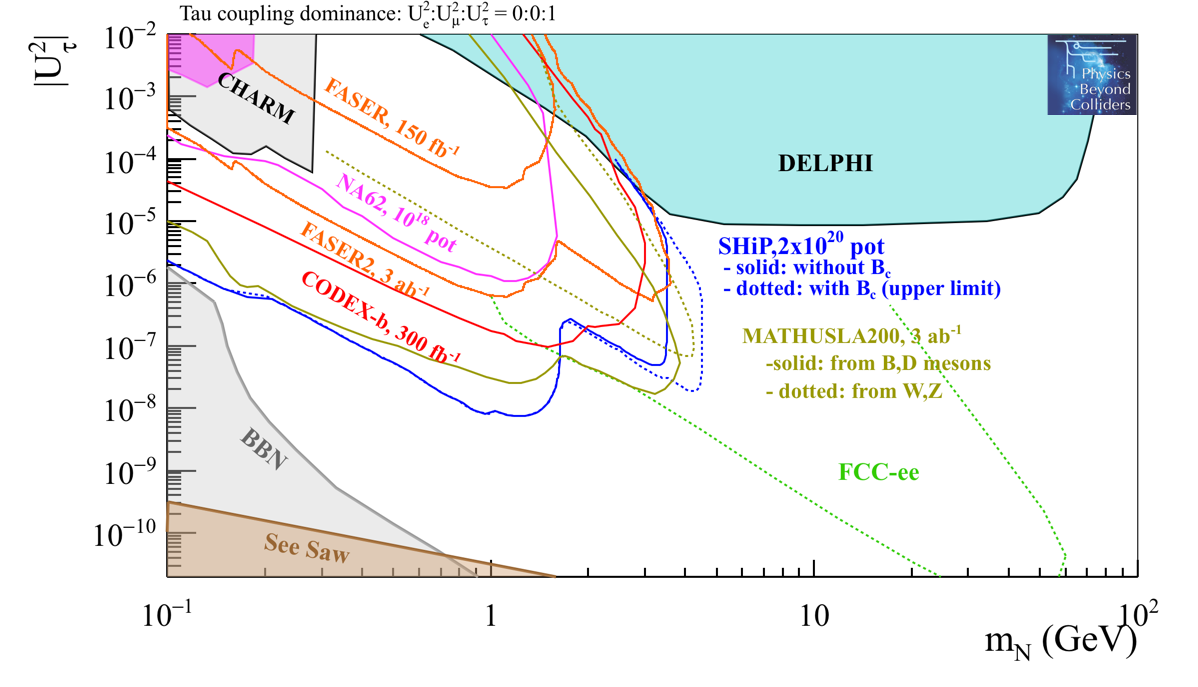
\includegraphics[width=.90\textwidth]{Figures/c3/HNL_bc8_pbc_2.png}
    \caption{Sensitivity to HNL with coupling to $\nu_\tau$ only. Current bounds (filled areas) and 10-15 years prospects for projects
(SHiP, MATHUSLA200, CODEX-b and FASER2) (solid lines). Projections from FCC-ee with $10^{12}$ $\PZ_0$ decays are also shown.}
  \label{fig:HNL_bc8_pbc_2}
\end{figure}

A brief experiment-focused overview follows:
\begin{itemize}
\item \textbf{PS191} (CERN, PS Beam 1983)~\cite{BERNARDI1988332}: the PS191
  experiment was specifically design to look for neutrino decays in
  low energy neutrino beam. It was a detector composed of a 12 m long
  decay volume followed by a fine-grain calorimeter. No sterile
  neutrino candidates were observed but the analysis of neutrino
  interactions in the calorimeter shows a possible excess of events
  with electrons~\cite{Vannucci:1985vs}.
\item \textbf{CHARM} (CERN, SPS beam 1985)~\cite{DORENBOSCH1986473}: A search
  for decays of HNL was performed by the CHARM Collaboration using a
  neutrino beam produced by dumping 400 GeV protons on a thick Copper
  target and looking for possible visible decays. It has been assumed
  the sterile neutrino to be produced by coupling in charmed D meson
  decays. The following decays were considered, \hnl $\rightarrow
  e^+e^-\nu_e$, $\rightarrow \mu^+e^-\nu_\mu$ and $\rightarrow
  \mu^+\mu^-\nu_\mu$ and the limits were settle on \mixpare and
  \mixparm $< \:10^{-7}$ for \hnl masses around 1.5 GeV. Neutrinos
  were assumed to be produced by neutral-current neutrino interactions
  in the CHARM calorimeter.
\item \textbf{Belle} (KEK, asymmetric-energy $e^+e^-$ collider, 2012)~\cite{Liventsev_2013}: Belle collaboration
  performed a search on heavy neutral leptons in B-meson
  decays. The data sample contained $772\times 10^6$ of $B\overline{B}$
  pairs collected at the $\Upsilon(4S)$ resonance. The limits
  on the mixing parameter were obtained analyzing the $B\overline{B}$ pairs
  events using the leptonic and semileptonic B meson decay,
  $B\rightarrow X\ell\nu_R$, where $\ell = e, \: \mu$ and the $X$ was
  either a charmed D meson, a light meson ($\pi, \: \rho, \: \eta$) or
  nothing (leptonic decay). Upper limits were set on on \mixpare and
  \mixparm in the mass range between 0.5-5.0 GeV. 
\item \textbf{DELPHI} (CERN, lepton collider LEP, 1997)~\cite{Abreu:1996pa}:
  the most stringent limits between 1 GeV and 10 GeV are still the ones
  been published by the DELPHI Collaboration. HNL search have been performed
  using the data collected by DELPHI detector corresponding to $3.3
  \times 10^6$ hadronic $Z_0$ decays at LEP1. These results are, up to
  this day, one of the most interesting and most complete because
  they include the short-lived HNL scenario and as well the long-lived
  HNL scenario. For short-lived, it was considered the \hnl production
  giving monojet or acollinear jet topologies, while for long-lived
  searchs, \hnl was looked for checking detectable secondary vertices or calorimeter clusters. 
 Upper limits were set for the branching ratio $BR, \: Z_0\rightarrow \hnl$ of
 about $1.3 \times 10^-6$ at 95\% C.L. for \hnl masses between 3.5 and
 50 GeV. 
\item \textbf{CMS and ATLAS} (CERN, LHC pp beam 2019): there have been several searches for HNLs in both CMS and ATLAS.
The ATLAS experiment recently reported on a search for HNLs using events with three charged leptons~\cite{atlasintro2} using 
pp collision data corresponding to integrated luminosities of 32.9 to
36.1 $fb^{-1}$. 
The search is performed in channels with three muons or two muons plus
one electron---providing sensitivity  to \mixparm only---, where the 
displaced decay vertex of the HNL was exploited.
CMS performed searches for HNLs only using prompt leptons,
either in final states with two same-charge leptons and one or two jets
(\(\PW^{\pm(\ast)}\to\ell^{\pm}\hnl\to\ell^{\pm}\ell^{\prime\pm}q\bar{q}^{\prime}\))~\cite{Sirunyan:2018xiv},
in a mass range of 20 GeV to 1.7 TeV.
CMS searches with three charged leptons in the final state using the leptonic \PW decay are going to extensively discussed in this
elaborate.
\end{itemize}

\subsection{Constraints on HNL}
In the following list, we tried so summarize the current constraints
coming from the theoretical predictions and from the most recent results (Figs.~\ref{fig:HNL_bc6_pbc_2},~\ref{fig:HNL_bc7_pbc_2}
and~\ref{fig:HNL_bc8_pbc_2}.)
\begin{itemize}
\item \textbf{Searches for Charged Lepton Flavor Violation}. If we consider an HNL with a
  mass close to EW scale and with large off-diagonal Yukawa couplings,
  then this type \hnl can lead to LFV in decays of charge leptons. Thus,
  testing LFV in multi-lepton searches could be an indirect way to
  probe the existence of HNL. Searches for such processes have
  placed 90\% C.L. upper limits on decay branching rates, \ie
  $BR(\mu^+\rightarrow e^+\gamma) < 4.2\times 10^{-13}$,
  $BR(\mu^+\rightarrow e^+e^+e^-) < 1.0\times 10^{-12}$ and
  $BR(\tau^-\rightarrow e^-\mu^+mu^-) < 2.7\times 10^{-8}$. For
  complete summary and references see~\cite{Pascoli_2019}.
\item \textbf{Cosmological constraints on light neutrino masses}. The Planck
  Satellite's measurements of the large scale structures in the
  universe, combined with the WMAP + highL + BAO data, have set the
  upper limits on the sum of all the light neutrino
  masses~\cite{Aghanim:2018eyx}: 
\begin{equation}
\label{eq:summasses}
\sum_{m} m_{\nu_m} < 0.12 \: eV, \;\;\;\; at \;95\% \: C.L.
\end{equation}
\item \textbf{BBN constraints}. Observing
  Figs.~\ref{fig:HNL_bc6_pbc_2},~\ref{fig:HNL_bc7_pbc_2}
  and~\ref{fig:HNL_bc8_pbc_2}, a \hnl which falls on the left of the
  Big Bag Nucleosynthesis line would be able to live long enough in
  the early Universe to cause an overproduction of primordial
  Helium-4~\cite{Ruchayskiy_2012}.
\item \textbf{Seesaw limit}. Below the line of the seesaw limit, the
  mixing of the sterile neutrinos with the active ones becomes too
  weak to be able to produce the pattern of neutrino flavor oscillations that has been observed~\cite{Canetti_2010}. 
\end{itemize}



\section{Summary}
\emph{to be re-written after}:
These few examples, which are going to be explored later on, show already the relevance and the interest of the HNL program and the strong motivations behind the existence of the $\nu_{R}$. This huge enthusiasm has lead in the past $\sim10$ years to the creation of a very active community with strong synergy between the theory people and the experimental collaborations which has brought to the publication of an impressive numbers of papers and the proposal of a consistent number of experiments focused manly on heavy neutral leptons. 






\clearpage

